\section{Theory}

By introducing an RC network across the Operational Amplifier, we can perform mathematical functions that include integration and differentiation. Because of the RC component, these circuits can also behave as filters and have a frequency response curve. 

In particular, op-amp filters are \textit{active filters}, meaning that due to the applied power source, they can apply additional gain to the signal. This is different from passive filters built using just resistors, capacitors and inductors, which attenuate the entire signal and hence the maximum gain one can achieve is 1.  

% ======================================================================================

\subsection{The Integrator Amplifier}

If the feedback resistor in an inverting amplifier is replaced by a capacitor as shown in Fig. \ref{int1}, the new op-amp circuit is known as an integrator.

\begin{figure}[H]
    \centering
    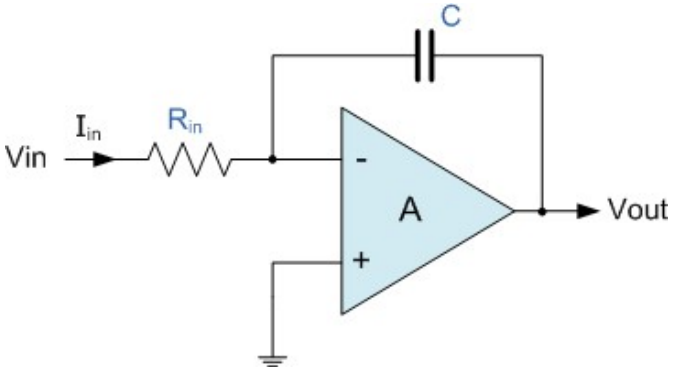
\includegraphics[width=0.6\columnwidth]{images/integrator.png}
    \caption{Integrator Circuit Diagram}
    \label{int1}
\end{figure}

When a voltage, \Xin{V} is firstly applied to the input, the uncharged capacitor $C$ has very little resistance and acts as a short circuit (voltage follower circuit) giving an overall gain of less than 1, thus resulting in zero output.
As the feedback capacitor begins to charge up, the ratio of $Z_f/$\Xin{R} increases producing an output voltage that continues to increase until the capacitor is fully charged. At this point the ratio $Z_f/$\Xin{R} is infinite resulting in infinite gain and the output of the amplifier goes into saturation (Fig.\ref{int2}).

\begin{figure}[H]
    \centering
    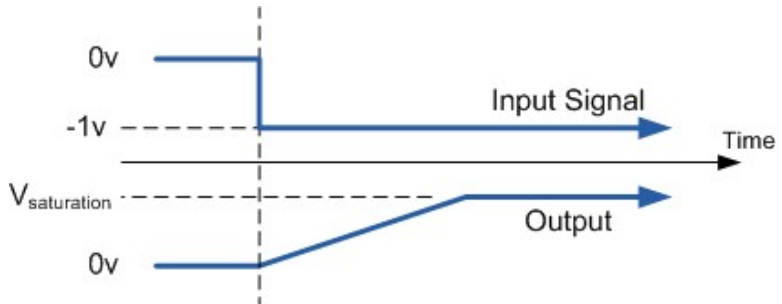
\includegraphics[width=0.9\columnwidth]{images/integrator_plot.png}
    \caption{Integrator circuit sample input and output curves}
    \label{int2}
\end{figure}

The rate at which the output voltage increases is determined by the RC time constant. By changing this value, the time in which it takes \Xout{V} to reach saturation can be changed.

Mathematically, we can express current flowing through the feedback capacitor as,

\begin{align}
    I_\text{in} = \frac{V_\text{in}}{R} &= -C\frac{V_\text{out}}{dt}\,\,\,\,(\because Q_\text{in}=CV_\text{out}) \nonumber\\
    \implies V_\text{out}(t) &= -\frac{1}{RC}\int V_\text{in}(t) \,dt 
\end{align}

Here, the gain can be expressed as,

\begin{align}
    A_V = -\frac{X_C}{R} \label{integrator_gain}
\end{align}

\begin{figure}[H]
    \centering
    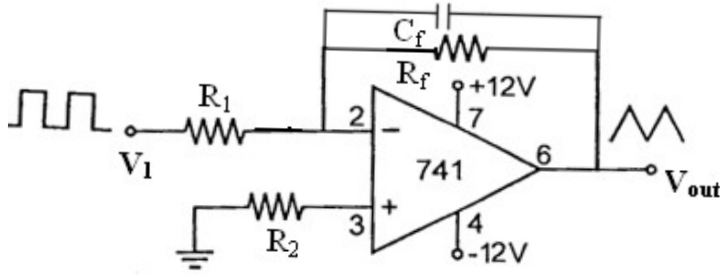
\includegraphics[width=0.9\columnwidth]{images/intcircuit.png}
    \caption{\textbf{Practical Integrator Circuit} with additional components -- (i) $R_f$ to produce stable biasing at DC and limits the gain of the circuit and (ii) $R_2$, which is the offset minimizing resistor which reduces output offset voltage due to input bias current}
    \label{intexp}
\end{figure}

% ======================================================================================

\subsection{Active Low Pass Filter}

From Eq. \ref{integrator_gain}, one can infer that as $f \rightarrow \infty$, $X_C \rightarrow 0$ and hence the gain $A_V \rightarrow 0$. Thus the circuit can attenuate high-frequency signals while letting low-frequency signal pass. However, the circuit behaves like a high-gain inverting amplifier at DC, when $f=0$. Hence it is viable to introduce a feedback resistance in parallel to the capacitor which produces stable biasing by restoring feedback at DC, so that the output voltage does not saturate.

\begin{figure}[H]
    \centering
    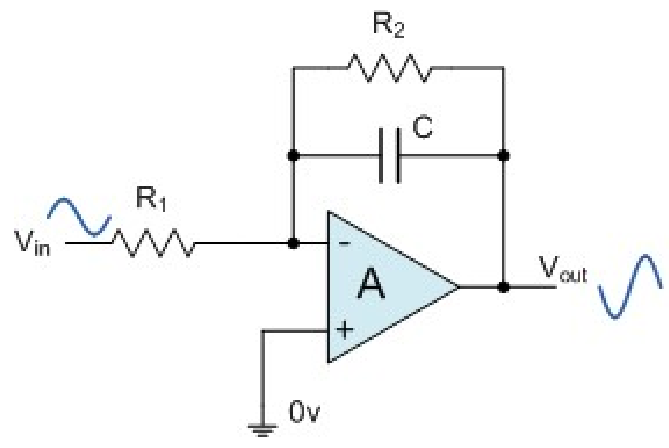
\includegraphics[width=0.6\columnwidth]{images/lowpass.png}
    \caption{Circuit diagram for an Active Low Pass Filter}
    \label{lowpasscircuit}
\end{figure}

Maximum gain is achieved when $f=0$, i.e. $A_V=R_2/R_1$. Hence, the frequency response would be something like Fig. \ref{lowpassbode}.

\begin{figure}[H]
    \centering
    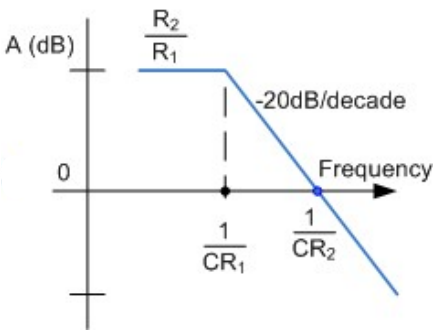
\includegraphics[width=0.6\columnwidth]{images/lowpassbode.png}
    \caption{Typical Frequency Response curve for an active low pass filer}
    \label{lowpassbode}
\end{figure}

% ======================================================================================

\subsection{The Differentiator Amplifier}

Here, the capacitor is connected to the input terminal of the inverting amplifier while the resistor, $R_f$ forms the negative feedback element across the operational amplifier. So the circuit produces an output voltage which is proportional to the rate-of-change of the input voltage and the current flowing through the capacitor.

\begin{figure}[H]
    \centering
    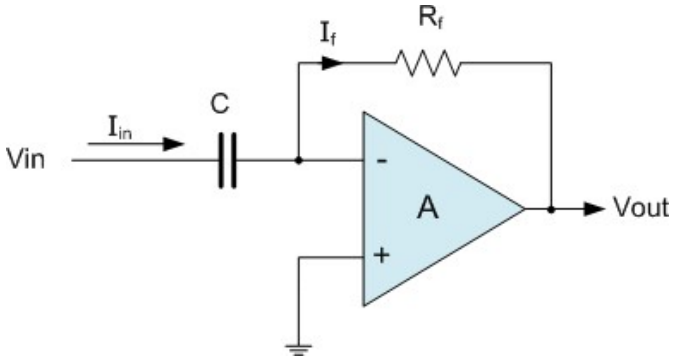
\includegraphics[width=0.7\columnwidth]{images/differentiator.png}
    \caption{Differentiator Circuit Diagram}
    \label{diff0}
\end{figure}

From the circuit (Fig. \ref{diff0}), we can express,

\begin{align}
    I_f=-\frac{V_\text{out}}{R_f}\text{ and }I_\text{in}=C\frac{dV_\text{in}}{dt}
\end{align}

Since we assume that no current passes through the op-amp,

\begin{align}
    I_f&=I_\text{in} \nonumber \\
    \implies V_\text{out} &= -R_f C\,\,\frac{dV_\text{in}}{dt}        
\end{align}

Hence, the output depends on the rate of change of the input signal. The gain of the amplifier is thus,

\begin{align}
    A_V=-\frac{R_f}{X_C} \label{differentiator_gain}
\end{align}

\begin{figure}[H]
    \centering
    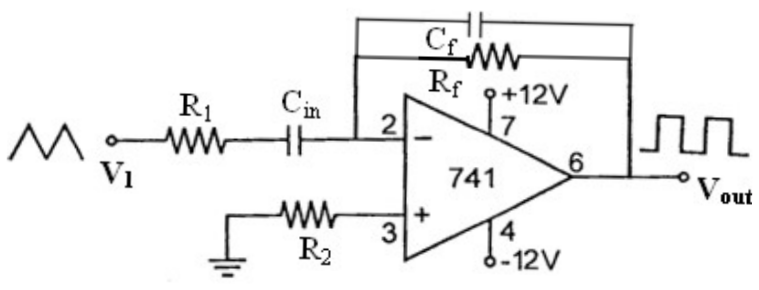
\includegraphics[width=0.90\columnwidth]{images/diffcircuit.png}
    \caption{\textbf{Practical Differentiator Circuit} with additional component -- (i) $C_f$ in parallel with $R_f$ to control gain at high frequencies, (ii) $R_1$ at the input in series with \Xin{C} to drop the noise at the input and (iii) $R_2$, the offset minimizing resistor which reduces output offset voltage due to input bias current}
    \label{diffexp}
\end{figure}


% ======================================================================================

\subsection{Active High Pass Filter}

Similar to the active low pass filter one can infer from Eq. \ref{differentiator_gain} that the gain is directly proportional to the frequency of the input signal. Thus the circuit can attenuate low-frequency signals while letting high-frequency signals pass. Thus, the capacitor blocks any DC content only allowing AC-type signals whose frequency is dependent on the rate of change of the input signal.

An ideal high pass filter will have a frequency response curve that looks like Fig. \ref{highpassbode}.

\begin{figure}[H]
    \centering
    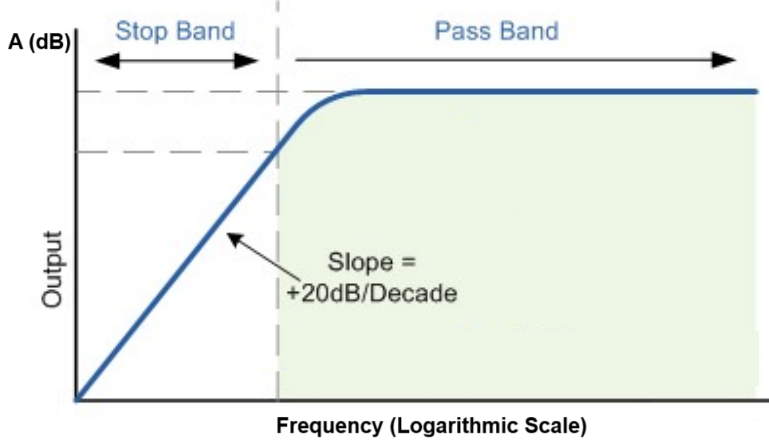
\includegraphics[width=0.8\columnwidth]{images/highpassbode.png}
    \caption{Typical frequency response curve of an active high pass filter}
    \label{highpassbode}
\end{figure}

Practically, the basic single resistor and single capacitor differentiator circuits are not widely used because of the two inherent faults -- Instability and Noise.

At high frequencies, a differentiator circuit becomes unstable and will start to oscillate. To avoid this, the high-frequency gain of the circuit needs to be reduced by adding an additional small value capacitor, $C_f$, across the feedback resistor $R_f$. Also, the capacitive input makes it very susceptible to random noise signals and any noise or harmonics present in the circuit will be amplified more than the input signal itself. This is because the output is proportional to the slope of the input voltage. So some means of limiting the bandwidth to achieve closed-loop stability is required. In order to reduce the overall closed-loop gain of the circuit at high frequencies, an extra Resistor, \Xin{R} is added to the input. Thus, the new circuit acts like a Differentiator amplifier at low frequencies and an amplifier with resistive feedback at high frequencies giving much better noise rejection (Fig. \ref{highpasscircuit}).

\begin{figure}[H]
    \centering
    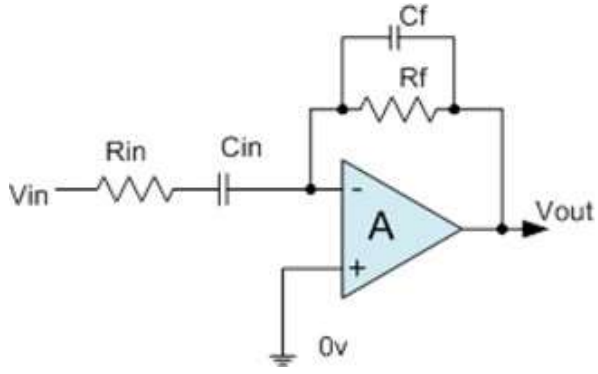
\includegraphics[width=0.7\columnwidth]{images/highpass.png}
    \caption{Circuit diagram for an Active High Pass Filter}
    \label{highpasscircuit}
\end{figure}

% ======================================================================================
\section{Experimental Setup}

\subsection*{Apparatus}

\begin{enumerate}
    \item OPAMP 741 Chip
    \item Resistors
    \item DC Power Supply
    \item Function Generator
    \item Breadboard
    \item Oscilloscope
    \item Connecting Wires
    \item Multimeters
\end{enumerate}

% \subsection*{Circuit Diagrams}
